% Created 2020-07-31 Fri 15:37
% Intended LaTeX compiler: pdflatex
\documentclass[presentation]{beamer}
\usepackage[utf8]{inputenc}
\usepackage[T1]{fontenc}
\usepackage{graphicx}
\usepackage{grffile}
\usepackage{longtable}
\usepackage{wrapfig}
\usepackage{rotating}
\usepackage[normalem]{ulem}
\usepackage{amsmath}
\usepackage{textcomp}
\usepackage{amssymb}
\usepackage{capt-of}
\usepackage{hyperref}
\usetheme{UoB}
\author{Mark Blyth}
\date{\textit{[2020-08-03 Mon]}}
\title{Surrogate models and novel discretisations}
\hypersetup{
 pdfauthor={Mark Blyth},
 pdftitle={Surrogate models and novel discretisations},
 pdfkeywords={},
 pdfsubject={},
 pdfcreator={Emacs 26.3 (Org mode 9.1.9)}, 
 pdflang={English}}
\begin{document}

\maketitle

\section{Last time}
\label{sec:org06928a5}
\begin{frame}[label={sec:org549a639}]{Last meeting}
\begin{itemize}
\item The challenges of working with spiking signals
\end{itemize}
\vfill
\begin{itemize}
\item Surrogate methods to overcome these
\end{itemize}
\end{frame}

\begin{frame}[label={sec:org7942ec0}]{Surrogates}
\begin{itemize}
\item Given \(y_i = f(x_i) + \varepsilon\), estimate \(f(x)\)
\end{itemize}
\vfill
\begin{itemize}[<+->]
\item Splines and Gaussian processes are good methods for estimation
\begin{itemize}
\item Gaussian point estimate: \(y \sim \mathcal{N}(f(x), \sigma^2_\varepsilon)\)
\item Gaussian function estimate: \(f(x) \sim \mathcal{GP}(\mu(x), k(x, x'))\)
\item Splines estimate: \(f_i(x) = a_0 + \dots + a_3x^3\), for \(x\in[\xi_i, \xi_{i+1})\)
\end{itemize}
\end{itemize}
\end{frame}

\section{Novel discretisations}
\label{sec:org9f06641}
\begin{frame}[label={sec:orgd45f45b}]{Developments since last time}
\begin{itemize}
\item Surrogates tested and working
\end{itemize}

\begin{center}
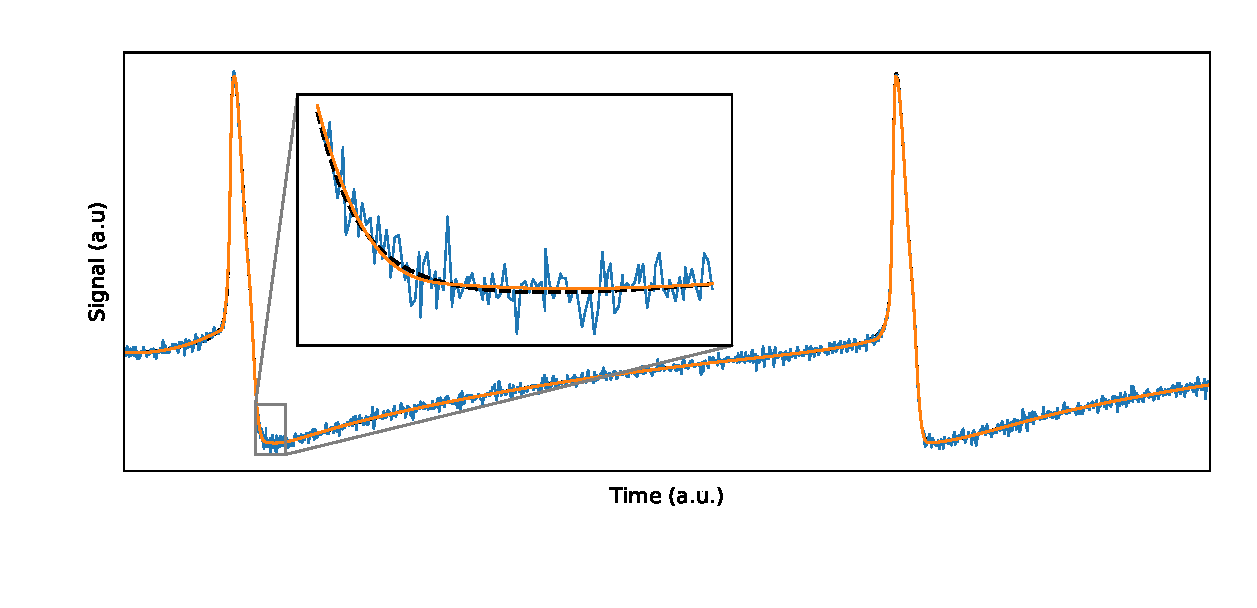
\includegraphics[width=.9\linewidth]{./surrogate.pdf}
\end{center}
\end{frame}

\begin{frame}[label={sec:orgc0f7230}]{Developments since last time}
\begin{itemize}
\item Testing novel discretisations
\end{itemize}
\vfill
\begin{itemize}
\item Implementing \emph{in-silico} CBC
\end{itemize}
\end{frame}

\begin{frame}[label={sec:org0c070ec}]{Discretisations}
\begin{itemize}
\item For \(f(x) = \sum \beta_i b_i(x)\), coefficients \(\{\beta_i\}\) discretise signal
\end{itemize}
\vfill
\begin{itemize}
\item Choose basis functions \(b_i(x)\) to minimise dimensionality
\end{itemize}
\end{frame}

\begin{frame}[label={sec:org5f10a53}]{Splines discretisation}
\begin{itemize}
\item Find a set of basis functions to initial signal \(f_0(x)\)
\begin{itemize}
\item Find \(\xi\) to optimise \(\{b_i(x)\}_\xi\) for \(f_0(x)\)
\end{itemize}
\end{itemize}
\vfill
\begin{itemize}
\item Discretisation of \(f_i(x)\) given by basis coefficients
\end{itemize}
\end{frame}

\begin{frame}[label={sec:orgf487fb7}]{Splines demo}
\begin{center}
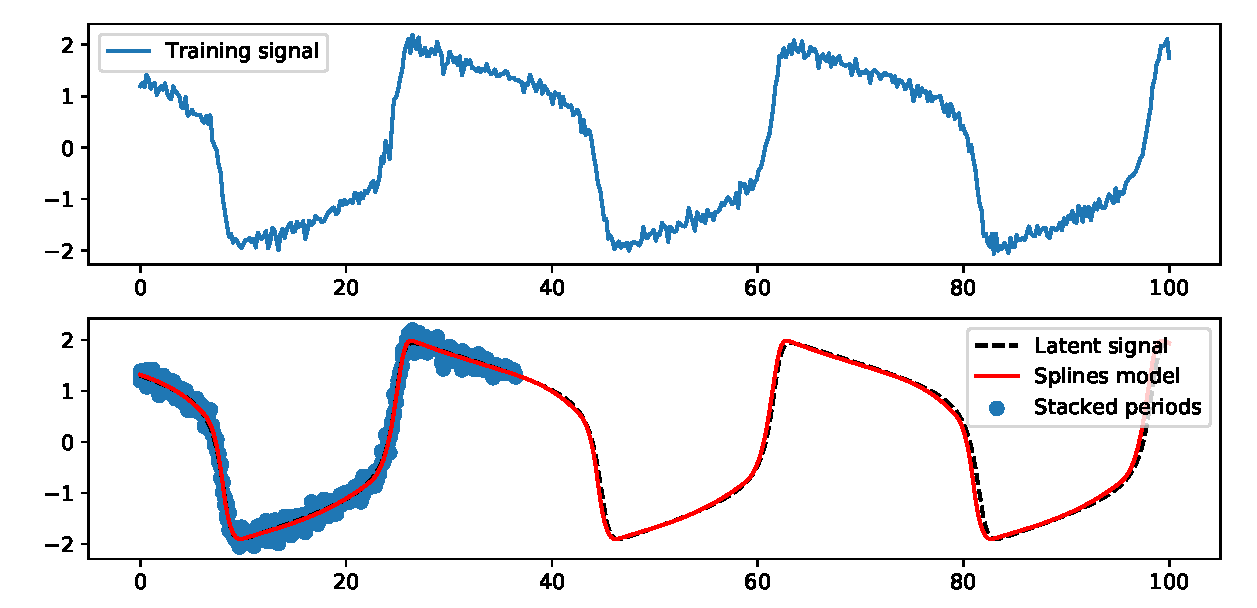
\includegraphics[width=.9\linewidth]{./spline_example.pdf}
\end{center}
\end{frame}

\begin{frame}[label={sec:org3e2c114}]{Splines vs Fourier}
\begin{center}
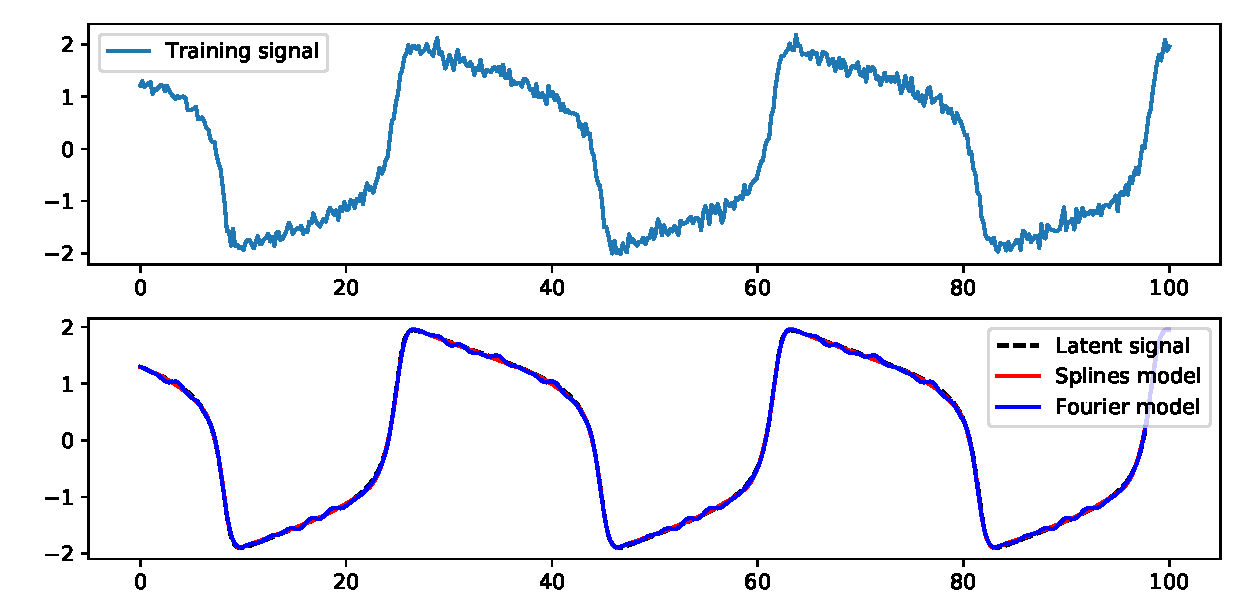
\includegraphics[width=.9\linewidth]{./discretisors.pdf}
\end{center}
\end{frame}

\begin{frame}[label={sec:org210f615}]{Goodness-of-fit}
\begin{center}
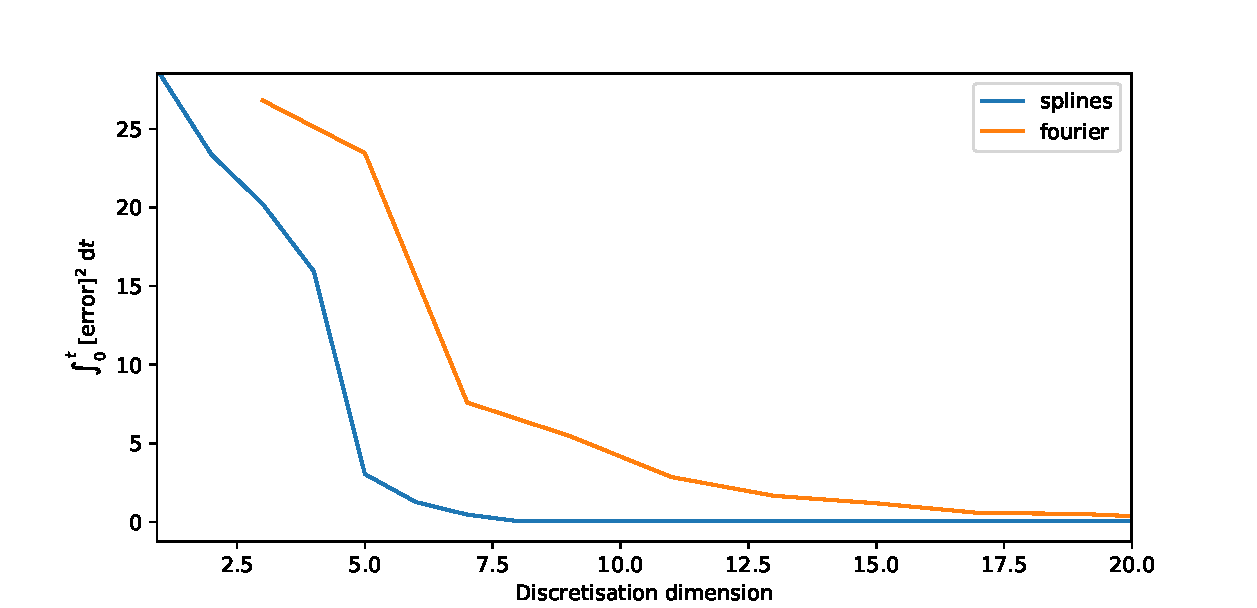
\includegraphics[width=.9\linewidth]{./goodness.pdf}
\end{center}
\end{frame}

\begin{frame}[label={sec:orgee48d66}]{Method usage cases}
Two approaches to CBC of periodic orbits:
\vfill
\begin{itemize}
\item Harmonically forced:
\begin{itemize}
\item Lump control action with bifurcation parameter; efficiently iterate Fourier harmonics to zero
\end{itemize}
\end{itemize}

\vfill
\begin{itemize}
\item Non-harmonically forced:
\begin{itemize}
\item Use Newton iterations to solve for noninvasive control action
\end{itemize}
\end{itemize}
\end{frame}

\section{CBC approach}
\label{sec:orgc4a3201}
\begin{frame}[label={sec:org8f76599}]{\emph{In-silico} CBC}
\begin{itemize}
\item Implement an in-silico CBC
\end{itemize}
\vfill
\begin{itemize}
\item Test it on a variety of toy models
\end{itemize}
\vfill
\begin{itemize}
\item Use it to demonstrate new discretisation
\end{itemize}
\end{frame}

\begin{frame}[label={sec:orgce51a2d}]{CBC method}
\begin{itemize}
\item Use PD control
\item Rescale periodics to \(t\in[0,1]\)
\item Non-adaptive mesh
\item Use Newton-iterations to solve for input = output
\end{itemize}
\end{frame}

\section{Code progress}
\label{sec:orgc474986}
\begin{frame}[fragile,label={sec:org0ccdcde}]{Discretisors}
 Discretisors implemented and lightly tested

\vfill

\begin{verbatim}
discretisation, period = discretisor.discretise(signal)

control_target = discretisor.undiscretise(
		    discretisation, period
)
\end{verbatim}
\end{frame}

\begin{frame}[fragile,label={sec:org90a3d81}]{Controllers}
 Controllers implemented and lightly tested

\begin{verbatim}
controller = Controller(
    "PD", B_matrix, control_target, 
    C_matrix=C_matrix, kp=10, kd=10
)
model = Model(
    fitzhugh_nagumo_neuron, ["I"], False, controller
)
solution = model.run_model(
    [0, 25], [-1, -1], I=1, rtol=1e-6
)  
\end{verbatim}
\end{frame}

\begin{frame}[label={sec:orgdceb19f}]{Control}
\begin{center}
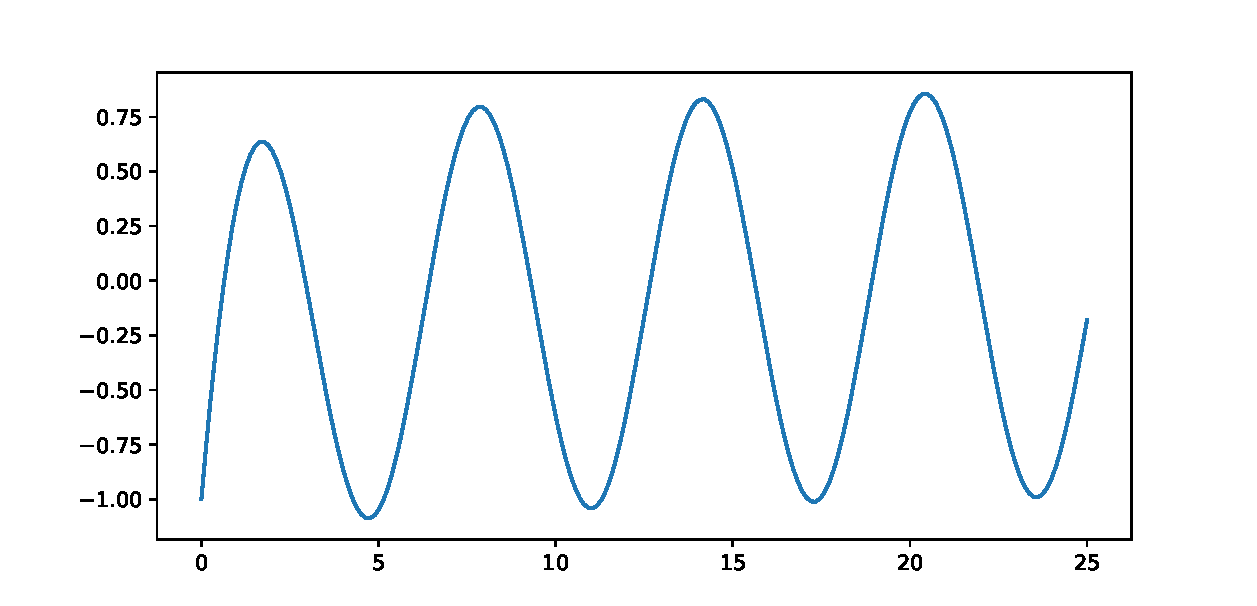
\includegraphics[width=.9\linewidth]{./controlled.pdf}
\end{center}
\end{frame}

\begin{frame}[fragile,label={sec:org953858b}]{Continuation}
 In progress; code written, but not tested

\vfill

\begin{verbatim}
next_orbit = prediction_correction_step(
	       system, po0, po1, stepsize, discretisor
)
\end{verbatim}
\end{frame}

\begin{frame}[label={sec:orgc6e2d45}]{Simulation summary}
\begin{itemize}
\item Control: implemented, lightly tested
\item Discretisation: implemented, lightly tested
\item Model-continuation interface: unimplemented
\item Continuation: implemented, untested
\item Results handling: unimplemented
\end{itemize}
\end{frame}

\section{Next steps}
\label{sec:org8c3db1e}
\begin{frame}[label={sec:org408c62b}]{Open questions}
\begin{itemize}
\item Will splines discretisation work?
\item Stationary or adaptive mesh?
\item Efficient solving methods?
\item Can we interface the code with Simulink?
\end{itemize}
\end{frame}



\begin{frame}[label={sec:orgd63fdef}]{Next steps}
\begin{itemize}
\item Finish CBC simulation
\item Start conference paper
\item Finish continuation review paper
\end{itemize}
\end{frame}
\end{document}
